\begin{homeworkProblem}
	\chapter{Architecture}
	\section{The Compiler}
	To give a quick overview of our compiler, we have a total of 8 modules:
	\begin{itemize}
		\item \textbf{analyzer.ml} - Semantically checks incoming AST representation to make sure that it includes existing files, adheres to the rules of inheritance, and expressions are properly type-checked
		\item \textbf{codegen.ml} - Converts a semantically checked AST into a working LLVM code by producing LLVM IR. 
		\item \textbf{dice.ml} - Main module that calls on all the other modules depending on compiler flags passed to it
		\item \textbf{filepath.ml} - Uses system calls to determine the absolute path to any file in the system. Useful for uniquely checking if an include statement refers to the same files
		\item \textbf{parser.mly} - Reads in tokens from the scanner to produce an AST representation of the program
		\item \textbf{processor.ml} - Handles communication between scanner and parser so that error messages regarding invalid input can be handled better
		\item \textbf{scanner.mll} - Reads a source file and tokenizes it to the corresponding token output. 
		\item \textbf{utils.ml} - Contains several functions for printing out the string representation of various intermediate representations in our language. Most critically used for debugging. 
	\end{itemize}
	
	and we have 4 interfaces
	\begin{itemize}
		\item \textbf{ast.ml} - Representation of program after parser
		\item \textbf{conf.ml} - Contains paths for accessing standard library and bindings
		\item \textbf{exceptions.ml} - All exceptions in the compiler
		\item \textbf{sast.ml} - The semantically checked representation of the language
	\end{itemize}
	
	and we have 2 library files
	\begin{itemize}
		\item \textbf{bindings.c} - A c file containing critical functions written in c that are usable in the language. This is compiled to LLVM bitcode and then linked with all source files compiled in our language
		\item \textbf{stdlib.dice} - A file containing user defined classes written in dice that are usable by the user
	\end{itemize}
	
	\subsection{The Scanner}
	The Scanner scans through the input file and tokenizes the input, discarding characters which are no longer need such as whitespace.
	
	\subsection{The Parser}
	The parser scans the tokens passed to it by the scanner and constructs an abstract syntax tree based on the definitions provided and the input tokens. The top level of the abstract syntax tree is a structure containing all classes and a structure containing all include statements. The Parser produces the following layout: 
	 \begin{figure}[!ht]
	 	\centering
	 	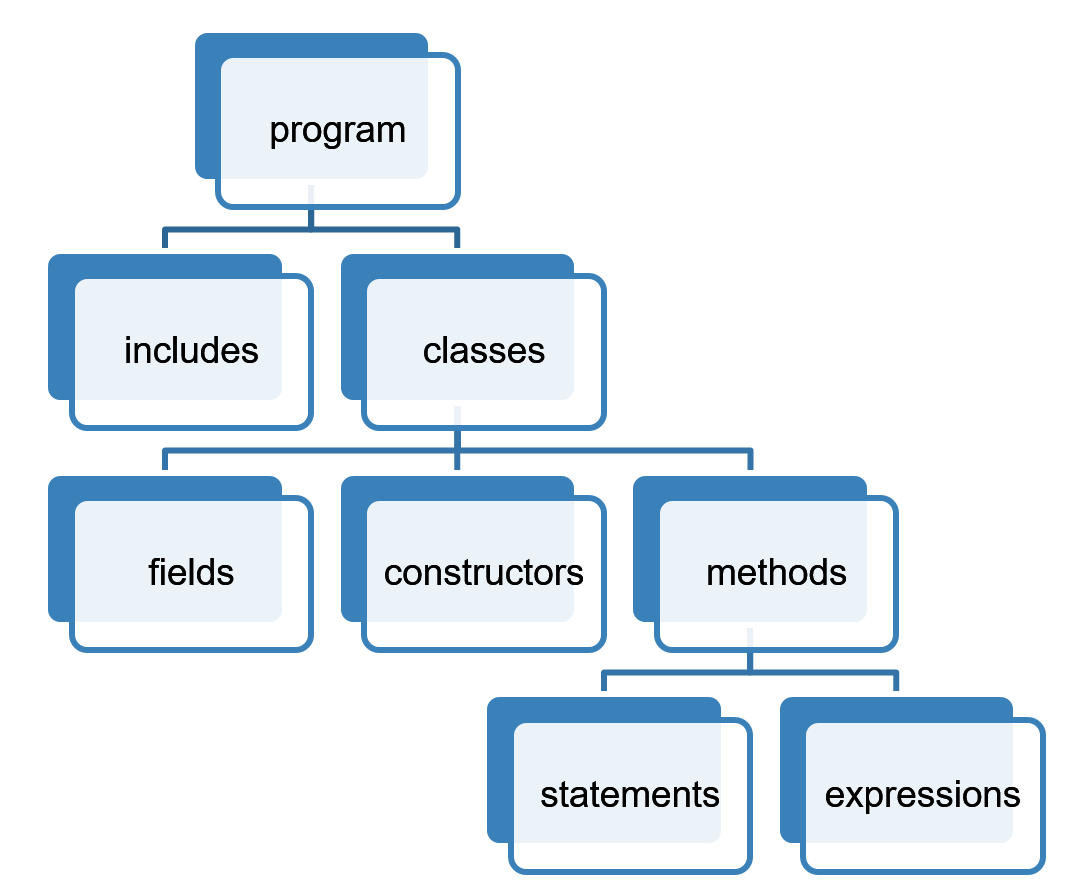
\includegraphics[width=4.5in]{Includes/ast}
	 	\caption{AST program representation.}
	 \end{figure}
	\subsection{The Semantic Analyzer}
	The first job of the Analyzer is to run the Scanner and Parser on any files contained in the includes statements of the given abstract syntax tree. The process of building an abstract syntax tree is the same for these files as for the originally compiled file. If any of these new abstract syntax trees contain include statements, the same process is run until there are no more includes. Similarly, each time a new included file's abstract syntax tree is passed to the Analyzer, all classes contained in the class structure of the new abstract syntax tree are appended to the original class list contained in the original class structure which was in the original abstract syntax tree. Once this process is complete, the analyzer is left with a class structure which contains every class defined in every file which was included with the originally compiled file.\\
	Next, the Analyzer performs an inheritance analysis by looking through the class list contained in the class structure and performs an analysis to determine whether any classes are children or parents of other classes. If there are any such relationships, the fields of each parent class are added to the front of its child's fields list, and the methods of each parent class are added to the child's method's list. However, if the child has declared a method or field which shares the same name as the parent's field or method, the child's field or method is not overwritten by the parent. As the inheritance analysis is performed, the list of fields for each class is also assigned a integer key beginning with 0 which will serve as the key to a lookup table which, at runtime, contains pointers to every function for each class.\\
	\begin{figure}[!ht]
		\centering
		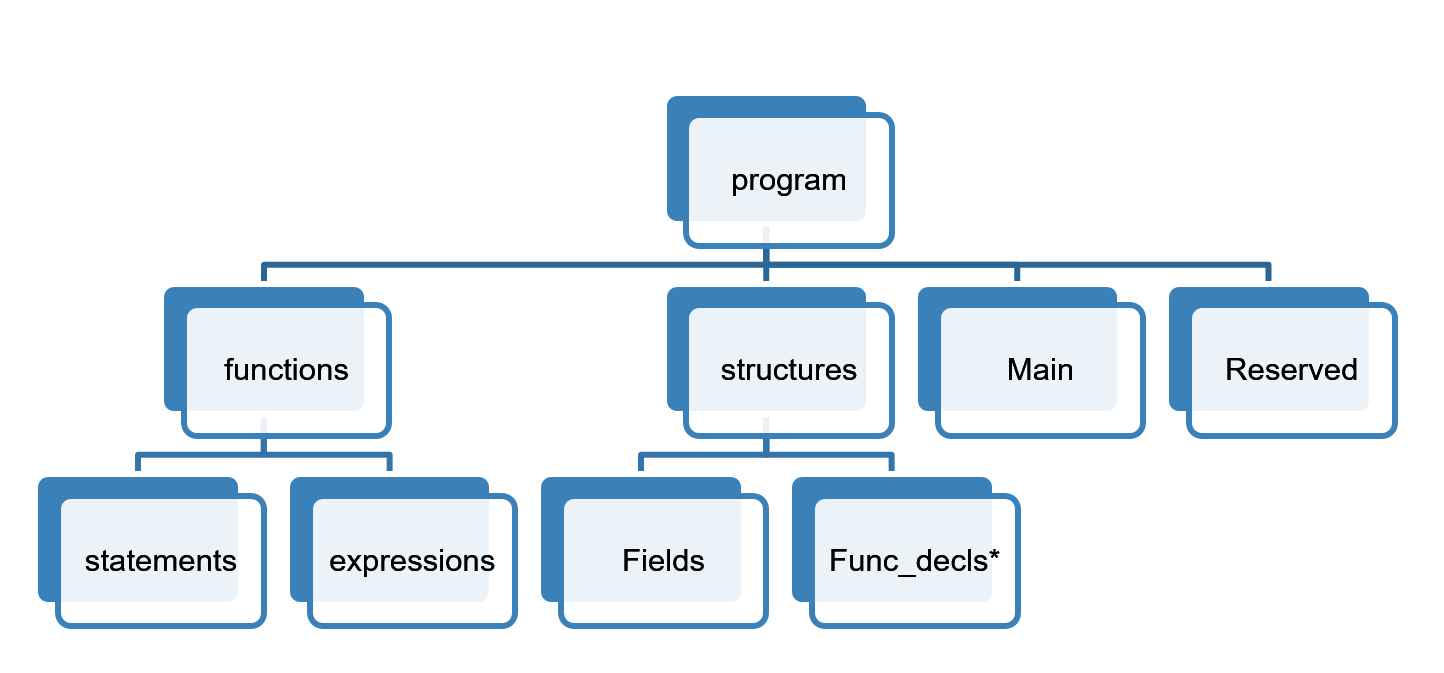
\includegraphics[width=4.5in]{Includes/sast}
		\caption{SAST representation.}
	\end{figure}
	Once the inheritance analysis is performed, semantic analysis is performed on each statement and expression in each block of code in every method for every class. This semantic analysis consists of making sure that types are consistent in every expression, making sure variables are declared and in the proper scope, and making sure that variables are only declared once. For instance, if an integer x is declared and x is assigned to the return of a method, the analyzer checks that the called method returns the type of x, namely an integer.\\
	As this analysis is performed, the analyzer is simultaneously constructing a semantic abstract syntax tree. The purpose of this new data structure is to provide the code generator with data that is organized more similarly to the LLVM code that it will eventually produce. Thus, instead of classes containing methods and fields, the top level program structure now contains separate sections for methods and fields. This is useful for the code generator because the LLVM code that is produced uses structs to store the fields of a class and functions to store the code within a class's methods. Thus, there is no inherent connection between the functions and the structs in LLVM. However, the analyzer modifies each method so that an instance of the structure containing the fields of the given class is passed in as the first argument to every function for that class. In this way, functions can access each field of a given class by accessing the data inside of the structure. 
	
	\subsection{The Code Generator}
    
    The code generator uses the semantic abstract syntax tree passed to it by the analyzer to construct the LLVM IR file which contains the final instructions for the program. \\
    
    \subsubsection{Structs and Inheritance}
    All structs are given an integer key at the beginning of their definition which will allow them to directly get their own virtual function table. Even if a subclass inherits from a parent class, it will be initialized with a specific key that is unique to the class at the beginning of each struct. For inherited fields they are organized in the order they were inherited, allowing multiple levels of inheritance. However it was too complex of a problem to solve multiple inheritance so we chose not to implement it. 
    \subsubsection{The Virtual Function Table}
	At compile time, an intermediate representation of the virtual function table is produced in LLVM IR. It is a function defined as "lookup" that is able to lookup a classes virtual function array by its class index and a function index unique to that function. The function index is generated from the Func\_decl list of a struct in the SAST. This way all subclasses have the same index for referring to the same function.
	\begin{figure}[!ht]
		\centering
		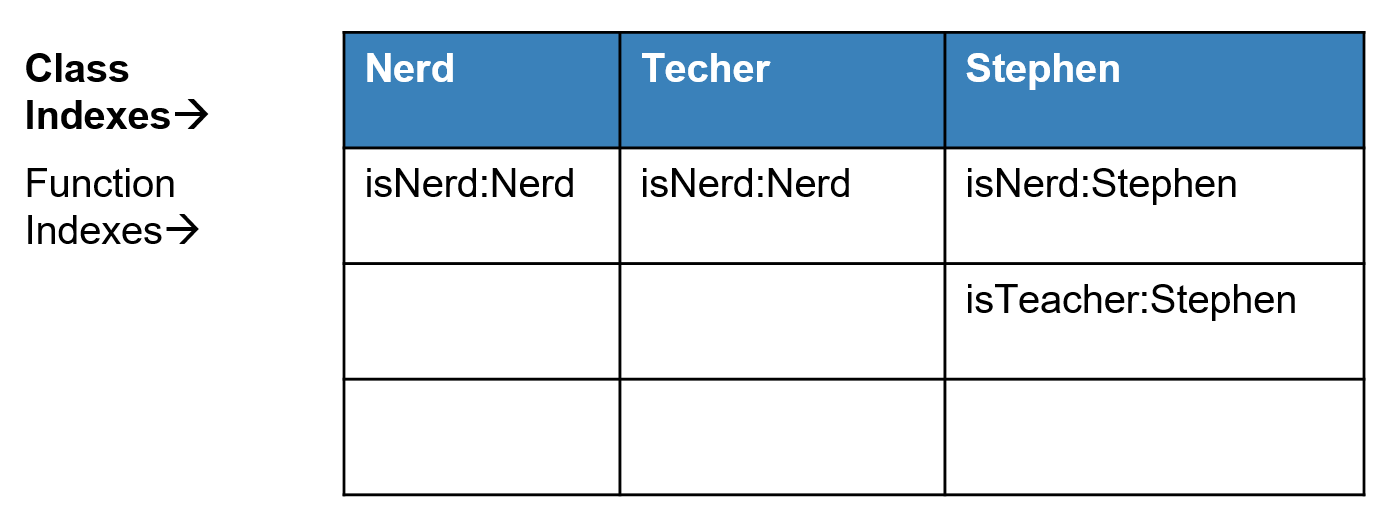
\includegraphics[width=4.5in]{Includes/vft}
		\caption{Virtual Function Table Example.}
	\end{figure}
	Take for example a class Nerd which has a subclass Techer, which itself has a subclass Stephen. Nerd has an isNerd method defined, Techer then inherits that method. Stephen would inherit that method but instead overrides them with its own implementation. But if a Nerd type variable is assigned to a Stephen type variable, the casted struct would still have the corresponding key to the Stephen class, and the function call would receive the correct index of 1 if isNerd were called. 
	\subsubsection{Expressions and Bindings}
	Once the inheritance code is generated, the code generator iterates through the entire semantic abstract syntax tree and produces the necessary LLVM code for each function, statement, and expression. This code generation is done using the OCaml LLVM library, which uses OCaml functions to produce the desired LLVM code.  We then link the resulting LLVM module with a precompiled bindings.bc which allows for the custom C functions we wrote to be incorporated into a user program in LLVM. 

	\subsection{The Utilities}
	Using the utils.ml module we were able to pretty print, print to JSON for AST and SAST, and print out the tokens for any given program. This made debugging the semantic analyzer much easier as we were able to see what went into it and what it produces at any time. The following is an example of what the SAST looks like in JSON.
	
	\begin{minted}[breaklines,linenos]{json}
{
	"sprogram": {
		"classes": [
		{ "scdecl": { "scname": "test", "sfields": [], "sfuncs": [] } }
		],
		"functions": [
		{
			"sfdecl": {
				"sfname": "test.constructor",
				"sreturnType": "class test",
				"sformals": [],
				"sbody": [
				{
					"slocal": {
						"datatype": "class test",
						"name": "this",
						"val": {
							"call": {
								"name": "cast",
								"params": [
								{
									"call": {
										"name": "malloc",
										"params": [
										{
											"call": {
												"name": "sizeof",
												"params": [
												{
													"id": {
														"name": "ignore",
														"datatype": "class test"
													}
												}
												],
												"index": 0,
												"datatype": "int"
											}
										}
										],
										"index": 0,
										"datatype": "char[]"
									}
								}
								],
								"index": 0,
								"datatype": "class test"
							}
						}
					}
				},
				{
					"sexpr": {
						"expr": {
							"assign": {
								"lhs": {
									"objaccess": {
										"lhs": {
											"id": { "name": "this", "datatype": "class test" }
										},
										"op": ".",
										"rhs": {
											"id": { "name": ".key", "datatype": "int" }
										},
										"datatype": "int"
									}
								},
								"op": "=",
								"rhs": { "int_lit": { "val": 0, "datatype": "int" } },
								"datatype": "int"
							}
						},
						"datatype": "int"
					}
				},
				{
					"sreturn": {
						"return": {
							"id": { "name": "this", "datatype": "class test" }
						},
						"datatype": "class test"
					}
				}
				],
				"func_type": "user"
			}
		}
		],
		"main": {
			"sfdecl": {
				"sfname": "main",
				"sreturnType": "void",
				"sformals": [
				{ "name": "this", "datatype": "class test" },
				{ "name": "args", "datatype": "char[][]" }
				],
				"sbody": [
				{
					"slocal": {
						"datatype": "class test",
						"name": "this",
						"val": {
							"call": {
								"name": "cast",
								"params": [
								{
									"call": {
										"name": "malloc",
										"params": [
										{
											"call": {
												"name": "sizeof",
												"params": [
												{
													"id": {
														"name": "ignore",
														"datatype": "class test"
													}
												}
												],
												"index": 0,
												"datatype": "int"
											}
										}
										],
										"index": 0,
										"datatype": "char[]"
									}
								}
								],
								"index": 0,
								"datatype": "class test"
							}
						}
					}
				},
				{
					"sexpr": {
						"expr": {
							"assign": {
								"lhs": {
									"objaccess": {
										"lhs": {
											"id": { "name": "this", "datatype": "class test" }
										},
										"op": ".",
										"rhs": { "id": { "name": ".key", "datatype": "int" } },
										"datatype": "int"
									}
								},
								"op": "=",
								"rhs": { "int_lit": { "val": 0, "datatype": "int" } },
								"datatype": "int"
							}
						},
						"datatype": "int"
					}
				},
				{
					"sexpr": {
						"expr": {
							"call": {
								"name": "print",
								"params": [
								{
									"string_lit": {
										"val": "Hello, World!",
										"datatype": "char[]"
									}
								}
								],
								"index": 0,
								"datatype": "void"
							}
						},
						"datatype": "void"
					}
				}
				],
				"func_type": "user"
			}
		},
		"reserved": [
		{
			"sfdecl": {
				"sfname": "print",
				"sreturnType": "void",
				"sformals": [ { "Many": "Any" } ],
				"sbody": [],
				"func_type": "reserved"
			}
		},
		{
			"sfdecl": {
				"sfname": "malloc",
				"sreturnType": "char[]",
				"sformals": [ { "name": "size", "datatype": "int" } ],
				"sbody": [],
				"func_type": "reserved"
			}
		},
		{
			"sfdecl": {
				"sfname": "cast",
				"sreturnType": "Any",
				"sformals": [ { "name": "in", "datatype": "Any" } ],
				"sbody": [],
				"func_type": "reserved"
			}
		},
		{
			"sfdecl": {
				"sfname": "sizeof",
				"sreturnType": "int",
				"sformals": [ { "name": "in", "datatype": "Any" } ],
				"sbody": [],
				"func_type": "reserved"
			}
		},
		{
			"sfdecl": {
				"sfname": "open",
				"sreturnType": "int",
				"sformals": [
				{ "name": "path", "datatype": "char[]" },
				{ "name": "flags", "datatype": "int" }
				],
				"sbody": [],
				"func_type": "reserved"
			}
		},
		{
			"sfdecl": {
				"sfname": "close",
				"sreturnType": "int",
				"sformals": [ { "name": "fd", "datatype": "int" } ],
				"sbody": [],
				"func_type": "reserved"
			}
		},
		{
			"sfdecl": {
				"sfname": "read",
				"sreturnType": "int",
				"sformals": [
				{ "name": "fd", "datatype": "int" },
				{ "name": "buf", "datatype": "char[]" },
				{ "name": "nbyte", "datatype": "int" }
				],
				"sbody": [],
				"func_type": "reserved"
			}
		},
		{
			"sfdecl": {
				"sfname": "write",
				"sreturnType": "int",
				"sformals": [
				{ "name": "fd", "datatype": "int" },
				{ "name": "buf", "datatype": "char[]" },
				{ "name": "nbyte", "datatype": "int" }
				],
				"sbody": [],
				"func_type": "reserved"
			}
		},
		{
			"sfdecl": {
				"sfname": "lseek",
				"sreturnType": "int",
				"sformals": [
				{ "name": "fd", "datatype": "int" },
				{ "name": "offset", "datatype": "int" },
				{ "name": "whence", "datatype": "int" }
				],
				"sbody": [],
				"func_type": "reserved"
			}
		},
		{
			"sfdecl": {
				"sfname": "exit",
				"sreturnType": "void",
				"sformals": [ { "name": "status", "datatype": "int" } ],
				"sbody": [],
				"func_type": "reserved"
			}
		},
		{
			"sfdecl": {
				"sfname": "getchar",
				"sreturnType": "int",
				"sformals": [],
				"sbody": [],
				"func_type": "reserved"
			}
		},
		{
			"sfdecl": {
				"sfname": "input",
				"sreturnType": "char[]",
				"sformals": [],
				"sbody": [],
				"func_type": "reserved"
			}
		}
		]
	}
}
	\end{minted}
	
	\section{Supplementary Code}
	\subsection{The Standard Library}
	The standard library was written in order to provide the user with a solid foundation on which to start writing interesting programs. To that end we provide for basic file i/o and string and integer manipulation.
	
	\subsection{String}
	Provide useful functionality for string manipulation.
	
	\subsubsection{Fields}
	String has no public fields. Private fields include a char array my\_string which stores the given string and an int to store the length of the string. 
	
	\subsubsection{Constructors}
	\paragraph{String(char[] a)}
	Accepts a char array, such as a string literal or a char array. This string is copied into the my\_string field of the object and the private length() method is run to get the length of the input string.
	
	\subsubsection{Methods}
	\paragraph{private int length\_internal(char[] input)}
	Returns the length of the given char array.
	\paragraph{private char[] copy\_iternal(char[] input)}
	Creates a new char array into which it copies the given char array.
	\paragraph{public char[] string()}
	Returns the char array contained in the my\_string field.
	\paragraph{public char getChar(int index)}
	Returns the char contained at the given index in the my\_string field.
	\paragraph{public int length()}
	Returns the length of the my\_string field
	\paragraph{public int toInteger()}
	Converts the char array in the my\_string field to an integer and returns that int. If the char array contained in the my\_string field is not a  string representation of an int, the behavior is undefined.
	\paragraph{public int toDigit(char digit)}
	Returns the integer corresponding to the character passed in.
	\paragraph{public class String copy(class String input)}
	Returns a copy of the current object.
	\paragraph{public int indexOf(char input)}
	Returns the index of the input character in the my\_string field. Returns -1 if the character is not found in the field.
	\paragraph{public class String reverse()}
	Returns a string object with the my\_string field containing the reverse of the current my\_string char array.
	\paragraph{public class String concat(class String temp)}
	Returns a string object with the my\_string field containing the concatenation of the current my\_string field with the temp's my\_string field.
	\paragraph{public bool compare(class String input)}
	Returns true if the my\_string field of the input String is equal to the my\_string field of the current String object.
	\paragraph{public bool contains(class String check)}
	Returns true if the my\_string field of the input String is contained in the my\_string field of the current String object.
	\paragraph{public void free()}
	Frees the memory for the my\_string field of the current String object.
	
	\subsection{File}
	The File class constructor takes two arguments: a char[] that points to an already opened file on which the user wishes to operate and a boolean indicating whether the user wishes to open the file for writing. If the boolean is true the file is opened for reading and writing, and if false the file is opened as read only. The constructor stores the given path in a field and then calls open() on the given path and, if successful, sets the object's file descriptor field to the return of open(). If open() fails, the program exits with error.
	\subsubsection{Fields}
	File has no public fields. Private fields are the class String filePath, private bool isWriteEnabled, and the private int fd.
	
	\subsubsection{Constructors}
	\paragraph{File(char[] path, bool isWriteEnabled)}
	Accepts a char array to open a file on, then creates a file object with the file descriptor. isWriteEnabled is a parameter that is used to determine whether the file can be written to or just read from.
	
	\subsubsection{Methods}
	\paragraph{private int openfile(class String path, bool isWriteEnabled)}
	Returns the file descriptor of the opened file if successful, and -1 otherwise. 
	\paragraph{public char[] readfile(int num)}
	Reads num bytes from the open file and returns the bytes in a char array.
	\paragraph{public int writefile(char[] arr, int offset)}
	Writes the contents of the char[] array to the file. If offset is -1 the write starts at the beginning of the file, if 0 it starts at the end of the file, and with any other positive integer it starts writing offset bytes from the beginning of the file.
	\paragraph{public void closefile()}
	Closes the open file. On error, the program exits with error.
	
	\subsection{Integer}
	The Integer class provides for integers to be converted to char arrays.
	\subsubsection{Fields}
	Integer has no public fields. There is one private field my\_int which stores the given integer.
	
	\subsubsection{Constructors}
	\paragraph{Integer(int input)}
	Accepts an integer which is stored in the field my\_int.
	
	\subsubsection{Methods}
	\paragraph{public int num()}
	Returns the integer stored in the my\_int field.
	\paragraph{public char toChar(int digit)}
	Returns in teh input digit as a character.
	\paragraph{public class String toString()}
	Converts the integer stored in the my\_int field into a string using the toChar() method. Returns a string object.
	\subsection{Built-in Functions}
	These are functions which are mapped from Dice to the C standard library, which is accessed through LLVM IR. The following function names may not be declared by the user since they are reserved. These are the only functions in dice which are not called as the method of an object; instead the user calls them directly with no dot operator.
	\subsubsection{int print(...)}
	The print function can take a char array, int, float and boolean. For char arrays, the contents of the array are printed to stdout. For every other type, the type is converted to the proper variable identifier as used in the C standard library printf function, and then the identifier is replaced with the value of the passed in type when the string is printed to standard out. Arguments can be in any order and must be comma separated.
	\subsubsection{char[] malloc(int size)}
	Returns a char pointer to an area of allocated memory on the heap of size bytes.
	\subsubsection{int open(char[] path)}
	Attempts to open the file located at the path specified and, if successful, returns a file descriptor to the open file. Returns -1 on failure.
	\subsubsection{int close(int fd)}
	Closes the open file identified by the integer fd. Returns 0 if successful and -1 on error.
	\subsubsection{int read(int fd, char[] buf, int num)}
	Reads num bytes from the open file identified by fd and stores the resulting string in the char array buf. If successful the number of bytes read is returned. Otherwise returns -1.
	\subsubsection{int write(int fd, char[] buf, int size)}
	Writes the contents of the char array buf, which contains size bytes, to the open file identified by fd. If successful the number of bytes written is returned. Otherwise returns -1.
	\subsubsection{int lseek(int fd, int offset, int whence)}
	The lseek() function repositions the offset of the open file associated with the file descriptor fd to the argument offset according to the directive whence as follows: 0 - the offset is set to offset bytes, 1 - The offset is set to its current location plus offset bytes, 2 - The offset is set to the size of the file plus offset bytes.
	\subsubsection{void exit(int flag)}
	Exits the program. Program exits without error is flag is 0 and exits with error if flag is set to any other integer.
	\subsubsection{int getchar()}
	Gets a character from stdin. Returns the character cast to an int.
	\subsection{Functions Implemented in C}
	With LLVM IR dice is able to compile functions written in C to LLVM. The following functions for dice were written in C.
	
	\subsection{Declarations}
	\subsubsection{char[] input()}
	The input function reads from stdin with the C standard library getchar() function, storing each character in a malloc'd char array, until a newline character is read. The resulting array is returned.
	\subsubsection{long[] init\_arr(int[] dims, int dimc)}
	Takes a list of dimensions in the form of ints and initialize a dimc-dimensional array in a one-dimension malloc call. To access element arr[1][2], first dereference a[1], and cast the value to a long*, which is an address to the array at position 1. Then dereference arr[2] and then cast that to a long* and the value is located at that position. This function is implemented in bindings.c, but was never incorporated directly into the language. 
\end{homeworkProblem}
